\documentclass[11pt, a4paper]{article}

\usepackage[top = 1 in, bottom = 1 in, left = 1 in, right = 1 in]{geometry}

\usepackage{amsmath}
\allowdisplaybreaks[1]
\usepackage{amssymb, amsfonts}
\usepackage{enumerate}
\usepackage{multirow}
\usepackage{hhline}
\usepackage{array}
\usepackage{longtable}
\usepackage{tikz}
\usepackage{mathrsfs}
\usepackage{graphicx}
\usepackage{tabularray}
\usepackage{dsfont}
\usepackage{undertilde}
\usepackage{dingbat}
\usepackage{latexsym}
\usepackage{fontawesome5}
\usepackage[colorlinks=true, linkcolor=blue, urlcolor=red]{hyperref}
\usepackage{tasks}
\usepackage{wrapfig}
\usepackage{bbding}
\usepackage{twemojis}
% how to use bull's eye ----- \scalebox{2.0}{\twemoji{bullseye}}
\usepackage{customdice}
% how to put dice face ------ \dice{2}
\usetikzlibrary{positioning}

\title{Backpropagation}
\author{Ananda Biswas}
\date{}



\begin{document}

\maketitle

\tableofcontents

\newpage

\section{Introduction}

Backpropagation is the core algorithm used to train neural networks. It is a method for computing the gradient of the loss function with respect to each of the weights and biases in the network, so we can use those gradients to adjust the weights and biases and minimize the loss (error). Recall that gradient descent or its upgradations require gradients of the loss function w.r.t. all the parameters of the model. Backpropagation is the very algorithm that provides the gradients. \\


Here we actually calculate the gradients of the loss with respect to each parameter (weight and bias) by applying the chain rule from the output layer back to the input layer. Starting from the input layer, when we move through the hidden layers and reach the output layer, it is called a \textbf{Forward-propagation}. Likewise when we traverse from the output layer, through the hidden layers back to the input layer, we call it a \textbf{Backward-propagation}.

\section{Set-up}

\begin{itemize}

\item Suppose we have a data-matrix $X_{n \times m}$ where $m$ is number of examples and $n$ is the number of features. [Generally, in a data-matrix, features construct the columns and examples are stacked vertically. Here we consider the transposed case \textit{i.e.} examples are in columns, it will help us in computation (linear algebra)].

\item Consider a fully connected Feed-forward neural network with 
	\begin{enumerate}[(i)]
	\item an input layer,
	\item $L - 1$ hidden layers 
	\item an output layer,
	\end{enumerate}	
each of these layers having some number of neurons.

\item Each neuron in the hidden layer and output layer can be split into two parts : 
	\begin{enumerate}[(i)]
	\item \textbf{pre-activation} or \textbf{aggregation} ($\utilde{a_i}$)
	\item \textbf{activation} ($\utilde{h_i}$).
	\end{enumerate}
	
\item The input layer is often called the 0-th layer and the output layer can be called the $L$-th layer.

\item $W_i$ and $\utilde{b_i}$ are the weights and biases between layers $i-1$ and $i$ $\forall i = 1(1)\overline{L-1}$. \\

$W_i \in \mathbb{R}^{n_{i} \times n_{i-1}}$ and $\utilde{b_i} \in \mathbb{R}^{n_{i}}$ where $n_{i}$ is the number of neurones at layer $i$. \\

Let the output layer have $p$ neurones. $W_L$ and $\utilde{b_L}$ are the weights and biases between the last hidden layer \textit{i.e.} layer $L-1$ and the output layer \textit{i.e.} layer $L$. \\

$W_L \in \mathbb{R}^{p \times n_{L-1}}$ and $\utilde{b_L} \in \mathbb{R}^{p}$.

\item $\forall i = 1(1)L$, pre-activation or aggregation at layer $i$ is given by
	$$\utilde{a_i} = W_i \cdot \utilde{h_{i-1}} + \utilde{b_i}$$
with $\utilde{h_0} = \utilde{x}$, the input.
	
\item $\forall i = 1(1)\overline{L-1}$
	\begin{itemize}
	\item activation at layer $i$ is given by
	$$\utilde{h_i} = g(\utilde{a_i})$$
	where $g(\cdot)$ is called the \textbf{activation function} for the hidden layers (\textit{e.g.} sigmoid, tanh, linear, ReLU etc.)
	
	\item activation at the output layer is given by
	$$ f(\utilde{x}) = \utilde{h_L}(\utilde{x}) = O(\utilde{a_L}(\utilde{x})) $$
	where $O(\cdot)$ is the output activation function (\textit{e.g.} softmax, linear, etc.)
	\end{itemize}

\item Obviously $\utilde{a_i}$s and $\utilde{h_i}$s are functions of $\utilde{x}$, the input.

\end{itemize}

\begin{figure}[!htbp]
\centering
\caption{A Feedforward Neural Network with $L = 3$ and $p = 2$}
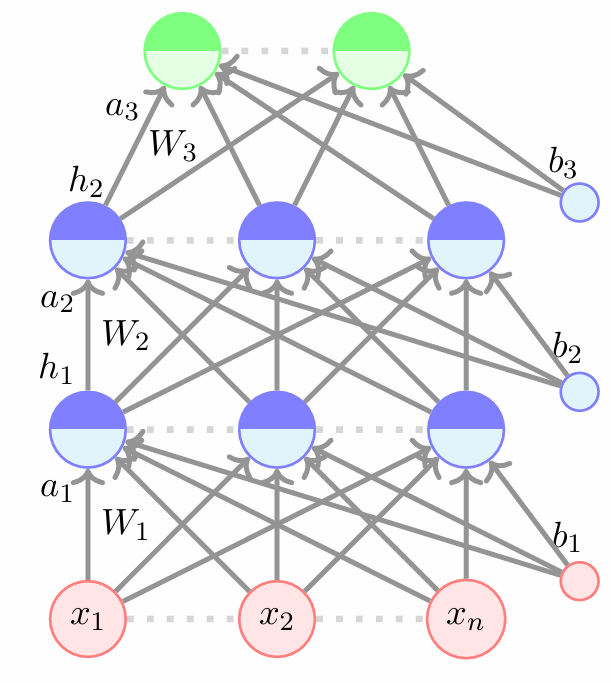
\includegraphics[scale=0.7]{image_1}
\label{fig:1}
\end{figure}


\section{Fundamentals}

The fundamental components for a Feedforward Neural Network are

\begin{enumerate}[(1)]

\item Data

\item Model

\item Parameters

\item Learning Algorithm

\item Loss Function

\end{enumerate}

Here we assume that we have a multi-class classification problem. \\

\leftpointright \hspace{0.1cm} We use \textbf{ReLU}$(g)$ at our hidden units and \textbf{Softmax}$(O)$ at the output units as activation functions; also we take \textbf{Average Sparse Categorical Cross-Entropy} as our loss function. \\

\leftpointright \hspace{0.1cm} If we stick with the architecture as in Figure~\ref{fig:1}, our neural network model will be

$$ \utilde{\hat{y}} = O(W_3 \cdot g(W_2 \cdot g(W_1 \cdot \utilde{x} + \utilde{b_1}) + \utilde{b_2}) + \utilde{b_3})$$

where $\utilde{\hat{y}} \in \mathbb{R}^{p \times 1}$ and our parameters will be $W_1, W_2, W_3, \utilde{b_1}, \utilde{b_2}, \utilde{b_3}$. \\

\leftpointright \hspace{0.1cm} Average Sparse Categorical Cross-Entropy Loss function is given by

$$L = \dfrac{1}{m} \sum \limits_{i = 1}^{m} - \log \hat{y_l}$$

where $\hat{y_l}$ is the predicted probability of true class $l$. \\

\leftpointright \hspace{0.1cm} The learning algorithm will be \textbf{gradient descent}. \\

So our Data, Model, Parameters and Loss Function is completely ready. In gradient descent (learning algorithm), we will need the gradients provided by backpropagation which is up next.


\section{Back-Propagation}

\subsection{Demo on a Thin Network}

\begin{wrapfigure}{r}{0.4\textwidth}
    \centering
    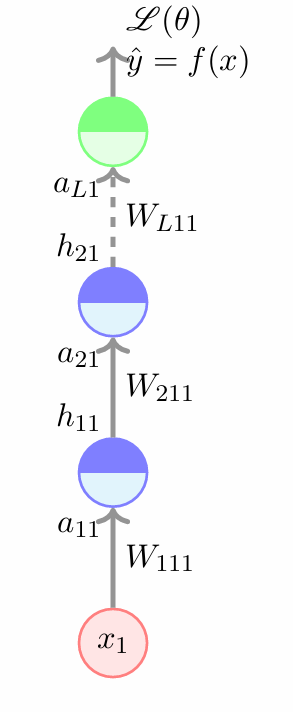
\includegraphics[scale = 0.6]{image_2.png}
    \caption{A Thin DNN}
    \label{fig:2}
\end{wrapfigure}

First let us take the simple case when we have a deep but thin network as in Figure~\ref{fig:2}. \\

$\bullet$ Let us focus on this weight $W_{111}$. To learn this weight using gradient descent we need a formula for $$\dfrac{\partial \mathscr{L}(\theta)}{\partial W_{111}}$$.

$\bullet$ By successive application of chain rule, we can do

$$\dfrac{\partial \mathscr{L}(\theta)}{\partial W_{111}} 
= \dfrac{\partial \mathscr{L}(\theta)}{\partial \hat{y}}
  \dfrac{\partial \hat{y}}{\partial a_{L11}}
  \dfrac{\partial a_{L11}}{\partial h_{21}}
  \dfrac{\partial h_{21}}{\partial a_{21}}
  \dfrac{\partial a_{21}}{\partial h_{11}}
  \dfrac{\partial h_{11}}{\partial a_{11}}
  \dfrac{\partial a_{11}}{\partial W_{111}}. $$

\subsection{Intuition}

Let us see an intuitive explanation of backpropagation before we get into the mathematical details. \\

Recall that derivative says how much a small change in $W_{111}$ changes $\mathscr{L}(\theta)$, in other words how much $W_{111}$ is responsible for the loss $\mathscr{L}(\theta)$. The less sensitive $W_{111}$ is, lesser will be the change in $\mathscr{L}(\theta)$ for a small change in $W_{111}$.


$\bullet$ We get a certain loss at the output and we try to figure out who is responsible for this loss.

\noindent
\begin{minipage}{0.45\textwidth}
    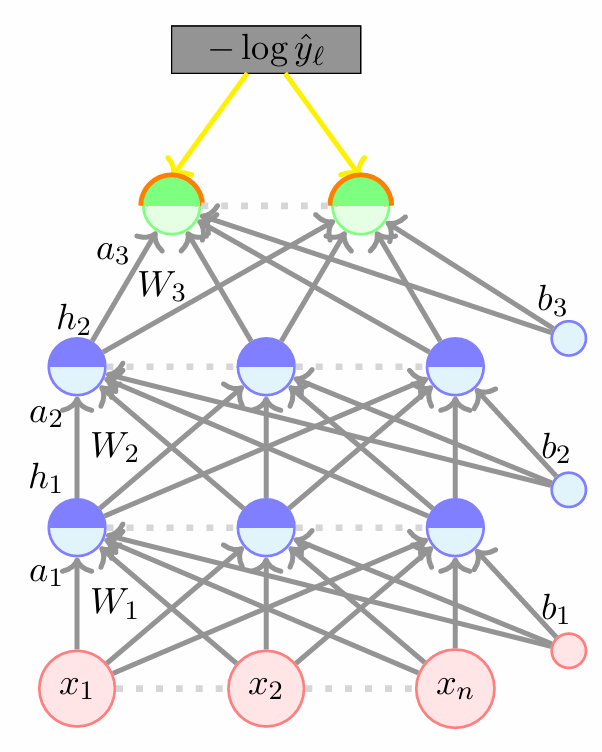
\includegraphics[scale = 0.5]{image_3.png}
\end{minipage}
\hfill
\begin{minipage}{0.5\textwidth}
    $\bullet$ So, we talk to the output layer and say ``Hey! You are not producing the desired output, better take responsibility."
\end{minipage}

\noindent
\begin{minipage}{0.5\textwidth}
    $\bullet$ The output layer says ``Well, I take responsibility for my part but please understand that I am only as the good as the hidden layer and weights below me. After all 
$$\hat{y} = O(W_L \cdot \utilde{h_{L-1}} + \utilde{b_L}).$$
So, we talk to $W_L, b_L$ and $h_L$ and ask them ``What is wrong with you ?"
\end{minipage}
\hfill
\begin{minipage}{0.45\textwidth}
    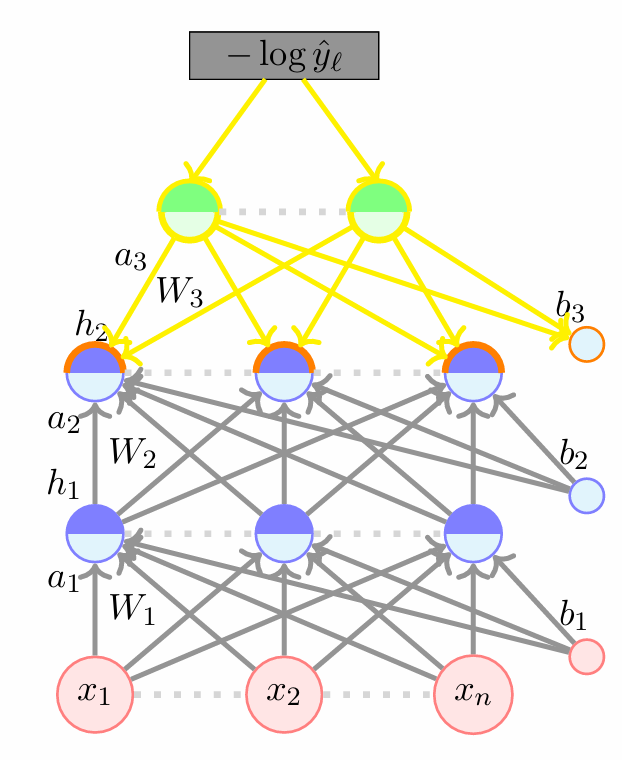
\includegraphics[scale = 0.5]{image_4.png}
\end{minipage}

\noindent
\begin{minipage}{0.45\textwidth}
    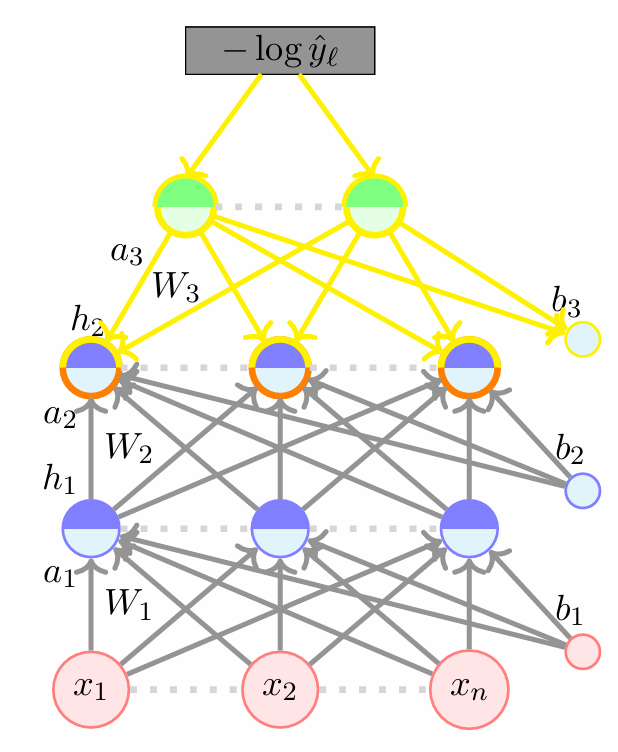
\includegraphics[scale = 0.49]{image_5.png}
\end{minipage}
\hfill
\begin{minipage}{0.5\textwidth}
    $\bullet$ $W_L$ and $b_L$ take full responsibility but $h_L$ says ``Well, please understand that I am only as good as the pre-activation layer."
\end{minipage}

\noindent
\begin{minipage}{0.5\textwidth}
    $\bullet$ The pre-activation layer in turn says that ``I am only as good as the hidden layer and weights below me."
\end{minipage}
\hfill
\begin{minipage}{0.45\textwidth}
    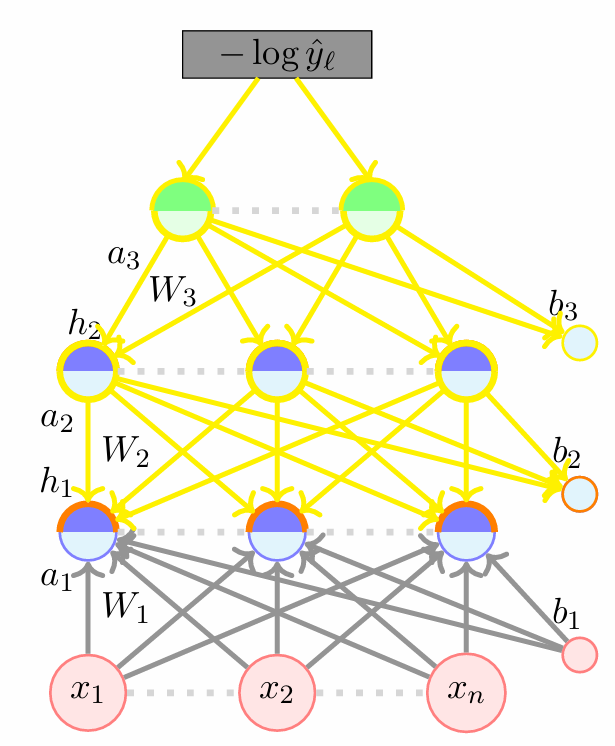
\includegraphics[scale = 0.5]{image_6.png}
\end{minipage}

\noindent
\begin{minipage}{0.45\textwidth}
    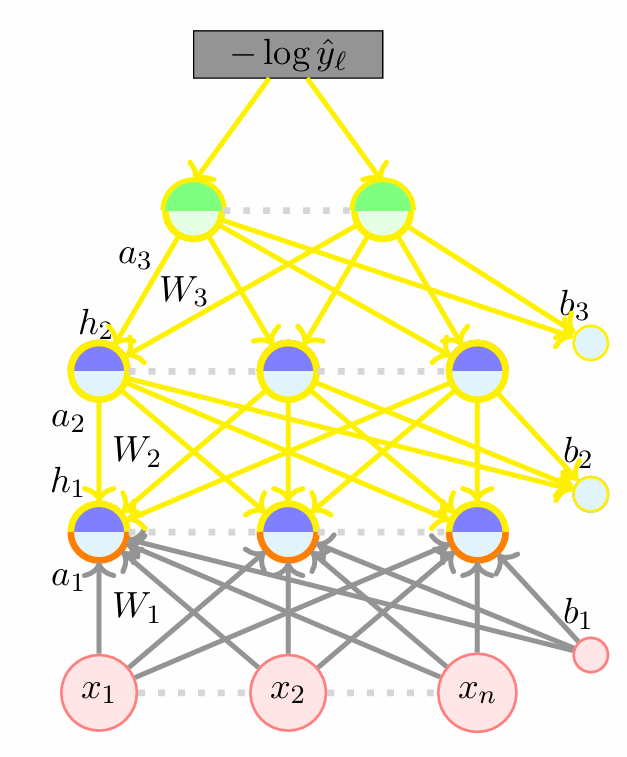
\includegraphics[scale = 0.49]{image_7.png}
\end{minipage}
\hfill
\begin{minipage}{0.5\textwidth}
    $\bullet$ We continue in this manner and realize that the responsibility lies with all the weights and biases (\textit{i.e.} all the parameters of the model).
\end{minipage}

\noindent
\begin{minipage}{0.5\textwidth}
    $\bullet$ But instead of talking to them directly, it is easier to talk to them through the hidden layers and output layers(and this is exactly what the chain rule allows us to do).
\end{minipage}
\hfill
\begin{minipage}{0.45\textwidth}
    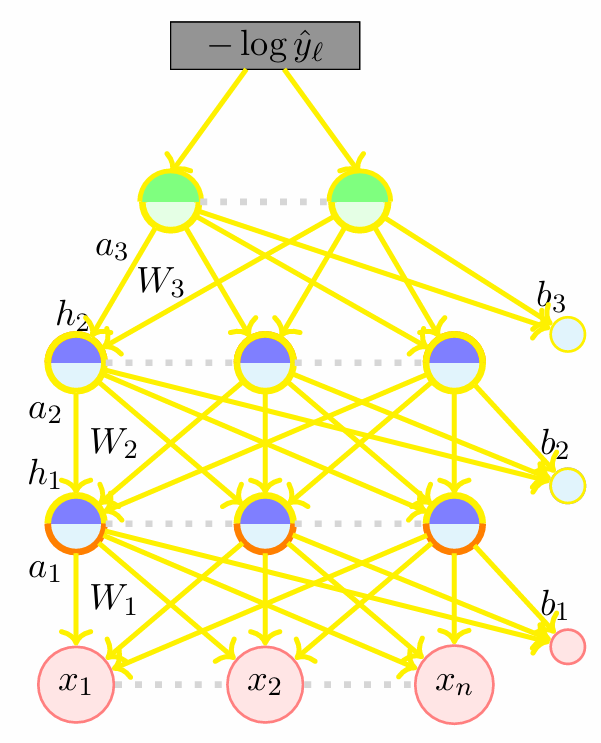
\includegraphics[scale = 0.5]{image_8.png}
\end{minipage}


$\spadesuit$ $$\underbrace{\dfrac{\partial \mathscr{L}(\theta)}{\partial W_{111}}}_{\shortstack{Talk to the\\weight directly}}
=
\underbrace{\dfrac{\partial \mathscr{L}(\theta)}{\partial \hat{y}} \dfrac{\partial \hat{y}}{\partial a_3}}_{\shortstack{Talk to the\\output layer}} \,\,\,\,\,\,
\underbrace{\dfrac{\partial a_3}{\partial h_2} \dfrac{\partial h_2}{\partial a_2}}_{\shortstack{Talk to the\\previous hidden\\layer}} \,\,\,\,\,\,
\underbrace{\dfrac{\partial a_2}{\partial h_1} \dfrac{\partial h_1}{\partial a_1}}_{\shortstack{Talk to the\\previous hidden\\layer}} \,\,\,\,\,\,
\underbrace{\dfrac{\partial a_1}{\partial W_{111}}}_{\shortstack{and now\\talk to\\the weights}}$$


\subsection{The Real Deal}

Here onwards our quantities of interest are

\begin{itemize}

\item gradients w.r.t. output units

\item gradients w.r.t. hidden units

\item gradients w.r.t. weights and biases

\end{itemize}

We first proceed assuming one data-point only, then we can always generalize for $m$ data-points.

\subsubsection{Gradients w.r.t. Output Units}

\vspace{0.3cm}

$$\underbrace{\dfrac{\partial \mathscr{L}(\theta)}{\partial W_{111}}}_{\shortstack{Talk to the\\weight directly}}
=
\textcolor{red}{\underbrace{\dfrac{\partial \mathscr{L}(\theta)}{\partial \hat{y}} \dfrac{\partial \hat{y}}{\partial a_3}}_{\shortstack{Talk to the\\output layer}}} \,\,\,\,\,\,
\underbrace{\dfrac{\partial a_3}{\partial h_2} \dfrac{\partial h_2}{\partial a_2}}_{\shortstack{Talk to the\\previous hidden\\layer}} \,\,\,\,\,\,
\underbrace{\dfrac{\partial a_2}{\partial h_1} \dfrac{\partial h_1}{\partial a_1}}_{\shortstack{Talk to the\\previous hidden\\layer}} \,\,\,\,\,\,
\underbrace{\dfrac{\partial a_1}{\partial W_{111}}}_{\shortstack{and now\\talk to\\the weights}}$$

\begin{gather*}
\utilde{\hat{y}} = 
\begin{pmatrix}
\hat{y_1} \\ \hat{y_2} \\ \hat{y_3} \\ \vdots \\ \hat{y_p}
\end{pmatrix}
\text{and }
\mathscr{L}(\theta) = - \log \hat{y_\ell} \,\, (\ell = \text{true class label})
\end{gather*}

Let us first consider the partial derivative w.r.t. $i$-th output.

\begin{align*}
\forall \,\, i = 1(1)p, \\[0.5em]
\dfrac{\partial}{\partial \hat{y_i}} \mathscr{L}(\theta) &= \dfrac{\partial}{\partial \hat{y_i}} (- \log \hat{y_\ell}) \\[0.5em]
&= \begin{cases}
\dfrac{1}{\hat{y_\ell}} \,\, \text{if } i = \ell \\[1em]
0 \,\, \text{otherwise}
\end{cases} \\[1em]
&= - \dfrac{\mathds{1}_{i = \ell}}{\hat{y_\ell}} \text{ where } \mathds{1}_{i = \ell} \text{ is an indicator function defined as } \mathds{1}_{i = \ell} = \begin{cases} 1 \text{ if } i = \ell \\ 0 \text{ otherwise } \end{cases}
\end{align*}

$\therefore \,\, \dfrac{\partial}{\partial \hat{y_i}} \mathscr{L}(\theta) = - \dfrac{\mathds{1}_{\ell = i}}{\hat{y_\ell}}.$
 
We can now talk about the gradient w.r.t. the vector $\utilde{\hat{y}}$ \textit{i.e.} $$\nabla_{\utilde{\hat{y}}} \mathscr{L}(\theta)$$ (it will be a collection of individual partial derivatives).

\begin{align*}
\nabla_{\utilde{\hat{y}}} \mathscr{L}(\theta) &= 
\begin{bmatrix}
\dfrac{\partial \mathscr{L}(\theta)}{\partial \hat{y_1}} \\[1em]
\dfrac{\partial \mathscr{L}(\theta)}{\partial \hat{y_2}} \\[1em]
\vdots \\[1em]
\dfrac{\partial \mathscr{L}(\theta)}{\partial \hat{y_p}}
\end{bmatrix} \\[0.5em]
&= - \dfrac{1}{\hat{y_\ell}} \begin{bmatrix}
\mathds{1}_{\ell = 1} \\[0.5em]
\mathds{1}_{\ell = 2} \\[0.5em]
\vdots \\[0.5em]
\mathds{1}_{\ell = p} \\[0.5em]
\end{bmatrix}
\begin{aligned}
& \bullet \text{train labels are one-hot encoded and at a time exactly one of the elements} \\ 
& \text{in this column vector is 1 and rest are 0.} \\
& \text{If } \ell \text{ is the true class label, then this column vector is equal to } \utilde{e_{\ell}} 
\end{aligned} \\[1em]
&= - \dfrac{1}{\hat{y_\ell}} \utilde{e_{\ell}} \, , \,\, \utilde{e_{\ell}} \text{ is a } p\text{-dimensional vector whose } \ell \text{-th element is 1 and rest are 0.}
\end{align*}

What we are actually interested in is

$$
\dfrac{\partial \mathscr{L}(\theta)}{\partial a_{Li}}
= \dfrac{\partial \, (- \log \hat{y_{\ell}})}{\partial a_{Li}}
= \dfrac{\partial \, (- \log \hat{y_{\ell}})}{\partial \hat{y_{\ell}}}\cdot \dfrac{\partial \hat{y_{\ell}}}{\partial a_{Li}} $$

and $\hat{y_{\ell}}$ indeed depends on $a_{Li}$ as $\hat{y_{\ell}} = \dfrac{exp \, (a_{L\ell})}{\sum \limits_{i = 1}^{p} exp \, (a_{Li})}$.


\begin{align*}
\text{Now, } \dfrac{\partial}{\partial a_{L i}} \left(- \log \hat{y}_\ell\right)
&= - \dfrac{1}{\hat{y}_\ell} \cdot \dfrac{\partial \hat{y}_\ell}{\partial a_{L i}} \\[1em]
&= - \dfrac{1}{\hat{y}_\ell} \cdot \dfrac{\partial}{\partial a_{L i}} \ \text{softmax}(\utilde{\mathbf{a}_L})_\ell \\[1em]
&= - \dfrac{1}{\hat{y}_\ell} \cdot \dfrac{\partial}{\partial a_{L i}} \left( \dfrac{\exp(\utilde{\mathbf{a}_L})_\ell}{\sum\limits_{i' = 1}^{p} \exp(\utilde{\mathbf{a}_L})_{i'}} \right), \text{ recall } \dfrac{\partial}{\partial x} \left(\dfrac{g(x)}{h(x)}\right)
= \dfrac{\dfrac{\partial g(x)}{\partial x} \cdot h(x) - g(x) \cdot \dfrac{\partial h(x)}{\partial x}}{\left(h(x)\right)^2} \\[1em]
&= - \dfrac{1}{\hat{y}_\ell} \cdot \left( \dfrac{\dfrac{\partial \exp(\utilde{\mathbf{a}_L})_\ell}{\partial a_{Li}}}{\sum\limits_{i' = 1}^{p} \exp(\utilde{\mathbf{a}_L})_{i'}} 
- \dfrac{\exp(\utilde{\mathbf{a}_L})_\ell \cdot \dfrac{\partial}{\partial a_{L i}} \sum\limits_{i' = 1}^{p} \exp(\utilde{\mathbf{a}_L})_{i'}}{\left( \sum\limits_{i' = 1}^{p} \exp(\utilde{\mathbf{a}_L})_{i'} \right)^2} \right) \\[1em]
&= - \dfrac{1}{\hat{y}_\ell} \cdot \left( \dfrac{\mathds{1}_{\ell = i} \exp(\utilde{\mathbf{a}_L})_\ell}{\sum\limits_{i' = 1}^{p} \exp(\utilde{\mathbf{a}_L})_{i'}} 
- \dfrac{\exp(\utilde{\mathbf{a}_L})_\ell \exp(\utilde{\mathbf{a}_L})_i}{\left( \sum\limits_{i' = 1}^{p} \exp(\utilde{\mathbf{a}_L})_{i'} \right)^2} \right) \\[1em]
&= - \dfrac{1}{\hat{y}_\ell} \cdot \left( \mathds{1}_{\ell = i} \ \text{softmax}(\utilde{\mathbf{a}_L})_\ell - \text{softmax}(\utilde{\mathbf{a}_L})_\ell \ \text{softmax}(\utilde{\mathbf{a}_L})_i \right) \\[1em]
&= - \dfrac{1}{\hat{y}_\ell} \cdot \left( \mathds{1}_{\ell = i} \ \hat{y}_\ell - \hat{y}_\ell \cdot \hat{y}_i \right) \\[1em]
&= - \left( \mathds{1}_{\ell = i} - \hat{y}_i \right)
\end{align*}

So far we have derived the partial derivative w.r.t. the $i$-th element of $\utilde{a_L}$ \textit{i.e.}

$$\dfrac{\partial \mathscr{L}(\theta)}{\partial a_{Li}} = - \left( \mathds{1}_{\ell = i} - \hat{y}_i \right).$$

We can now write the gradient w.r.t. the vector $\utilde{a_L}$.

\begin{align*}
\nabla_{\mathbf{\utilde{a_L}}} \mathscr{L}(\theta)
&= \begin{bmatrix}
\dfrac{\partial \mathscr{L}(\theta)}{\partial a_{L1}} \\[1.5em]
\dfrac{\partial \mathscr{L}(\theta)}{\partial a_{L2}} \\[1.5em]
\vdots \\[1.5em]
\dfrac{\partial \mathscr{L}(\theta)}{\partial a_{Lp}}
\end{bmatrix} \\[2.5em]
&= \begin{bmatrix}
- \left( \mathds{1}_{\ell = 1} - \hat{y}_1 \right) \\[1.5em]
- \left( \mathds{1}_{\ell = 2} - \hat{y}_2 \right) \\[1.5em]
\vdots \\[1.5em]
- \left( \mathds{1}_{\ell = p} - \hat{y}_p \right)
\end{bmatrix} \\[2.5em]
&= - \left( \utilde{e_{\ell}} - \utilde{\hat{y}} \right)
\end{align*}



\subsubsection{Gradients w.r.t. Hidden Units}

\vspace{0.3cm}

$$\underbrace{\dfrac{\partial \mathscr{L}(\theta)}{\partial W_{111}}}_{\shortstack{Talk to the\\weight directly}}
=
\underbrace{\dfrac{\partial \mathscr{L}(\theta)}{\partial \hat{y}} \dfrac{\partial \hat{y}}{\partial a_3}}_{\shortstack{Talk to the\\output layer}} \,\,\,\,\,\,
\textcolor{red}{\underbrace{\dfrac{\partial a_3}{\partial h_2} \dfrac{\partial h_2}{\partial a_2}}_{\shortstack{Talk to the\\previous hidden\\layer}}} \,\,\,\,\,\,
\textcolor{red}{\underbrace{\dfrac{\partial a_2}{\partial h_1} \dfrac{\partial h_1}{\partial a_1}}_{\shortstack{Talk to the\\previous hidden\\layer}}} \,\,\,\,\,\,
\underbrace{\dfrac{\partial a_1}{\partial W_{111}}}_{\shortstack{and now\\talk to\\the weights}}$$

$\bullet$ \textbf{Chain Rule along multiple paths : } If a function $p(z)$ can be written as a function of intermediate results $q_i(z)$, then we have :

$$\dfrac{\partial p(z)}{\partial z} = \sum \limits_{m} \dfrac{\partial p(z)}{\partial q_m(z)} \cdot \dfrac{\partial q_m(z)}{\partial z}$$

Here is an example.

\begin{center}
\begin{minipage}{0.5\textwidth}
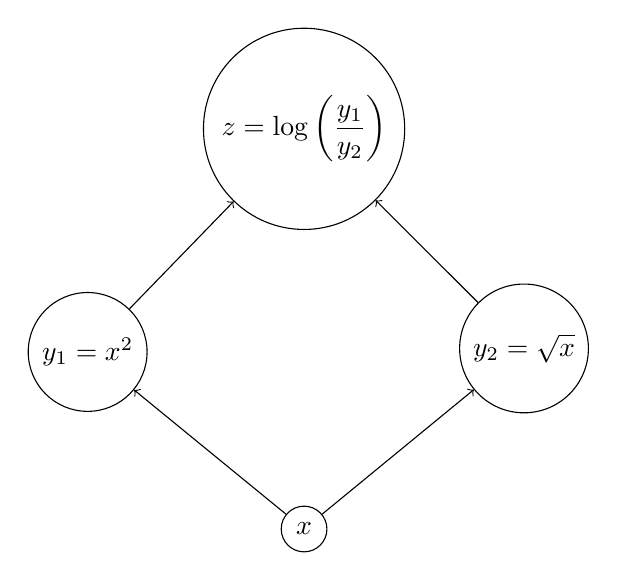
\begin{tikzpicture}[node distance=2cm]

% Nodes
\node (x) [circle, draw] {$x$};
\node (y1) [circle, draw, above left=1.5cm and 2cm of x] {$y_1 = x^2$};
\node (y2) [circle, draw, above right=1.5cm and 2cm of x] {$y_2 = \sqrt{x}$};
\node (z)  [circle, draw, above=3.5cm of x] {$z = \log\left(\dfrac{y_1}{y_2}\right)$};

% Arrows
\draw[->] (x) -- (y1);
\draw[->] (x) -- (y2);
\draw[->] (y1) -- (z);
\draw[->] (y2) -- (z);

\end{tikzpicture}
\end{minipage}
\hfill
\begin{minipage}{0.4\textwidth}
\[
\dfrac{dz}{dx} = \sum_{i=1}^{2} \dfrac{dz}{dy_i} \cdot \dfrac{dy_i}{dx}
\]
\end{minipage}
\end{center}



\noindent
\begin{minipage}{0.5\textwidth}
    First, 
\begin{align*}
\dfrac{\partial \mathscr{L}(\theta)}{\partial h_{ij}} &= \sum \limits_{m = 1}^{p} \dfrac{\partial \mathscr{L}(\theta)}{\partial a_{i+1, m}} \cdot \dfrac{\partial a_{i+1, m}}{\partial h_{ij}} \\[1.5em]
&= \sum \limits_{m = 1}^{p} \dfrac{\partial \mathscr{L}(\theta)}{\partial a_{i+1, m}} \cdot W_{i+1, m, j} \,\, \text{as } \utilde{a_{i+1}} = W_{i+1} \utilde{h_i} + \utilde{b_{i+1}}\\[1.5em]
\end{align*}
\end{minipage}
\hfill
\begin{minipage}{0.45\textwidth}
    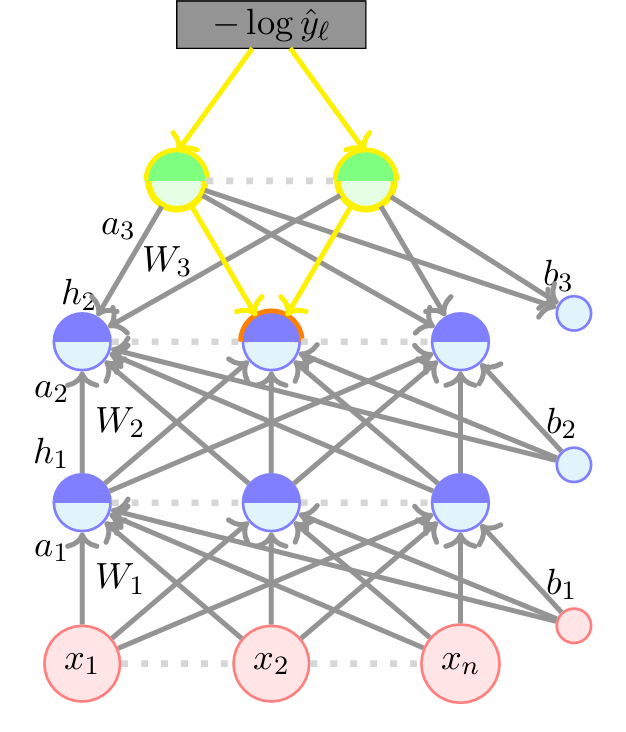
\includegraphics[scale = 0.5]{image_9.png}
\end{minipage}


Now consider these two vectors,

\[
\nabla_{a_{i+1}} \mathscr{L}(\theta) =
\begin{bmatrix}
\dfrac{\partial \mathscr{L}(\theta)}{\partial a_{i+1,1}} \\
\vdots \\
\dfrac{\partial \mathscr{L}(\theta)}{\partial a_{i+1,k}}
\end{bmatrix}
\quad ; \quad
W_{i+1,\cdot,j} =
\begin{bmatrix}
W_{i+1,1,j} \\
\vdots \\
W_{i+1,k,j}
\end{bmatrix}
\]

\vspace{0.2cm}

$W_{i+1,\cdot,j}$ is the $j$-th column of $W_{i+1}$; see that,

\[
\left(W_{i+1,\cdot,j}\right)^T \nabla_{a_{i+1}} \mathscr{L}(\theta)
=
\sum_{m=1}^{k} \dfrac{\partial \mathscr{L}(\theta)}{\partial a_{i+1,m}} W_{i+1,m,j}
\]

\vspace{0.2cm}

We have,
\[
\dfrac{\partial \mathscr{L}(\theta)}{\partial h_{ij}} = \left(W_{i+1,\cdot,j}\right)^T \nabla_{a_{i+1}} \mathscr{L}(\theta)
\]

\vspace{0.2cm}

\begin{table}
\def\arraystretch{1.5}

\begin{center}
\begin{tabular}{cc}
\centering
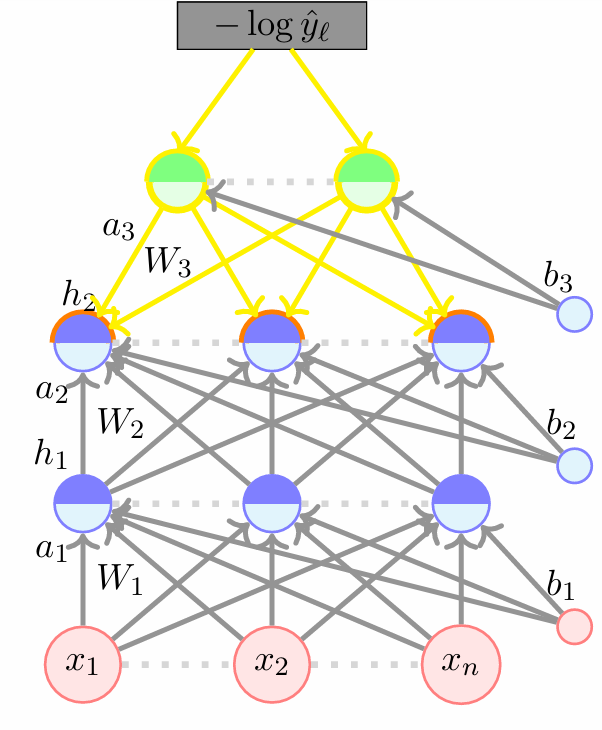
\includegraphics[scale = 0.5]{image_10.png}
&
\centering
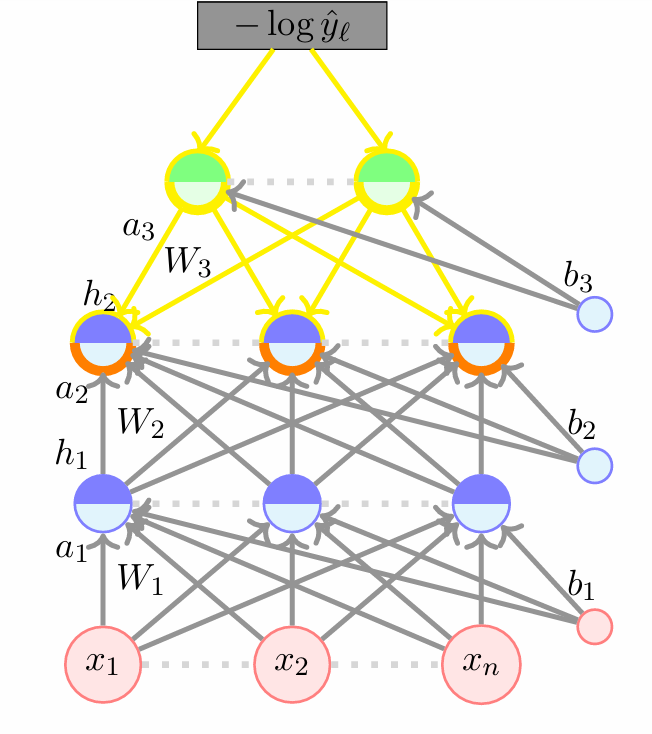
\includegraphics[scale = 0.5]{image_11.png}

\end{tabular}
\caption{Gradients w.r.t. hidden layers}
\label{tab:1}
\end{center}
\end{table}


We can now write the gradient w.r.t. $\utilde{h_i}$ (left figure in Table~\ref{tab:1}).

\begin{align*}
\nabla_{\mathbf{h}_i} \mathscr{L}(\theta)
=
\begin{bmatrix}
\dfrac{\partial \mathscr{L}(\theta)}{\partial h_{i1}} \\[1em]
\dfrac{\partial \mathscr{L}(\theta)}{\partial h_{i2}} \\[1em]
\vdots \\[1em]
\dfrac{\partial \mathscr{L}(\theta)}{\partial h_{in}}
\end{bmatrix}
=
\begin{bmatrix}
\left(W_{i+1,\cdot,1}\right)^T \nabla_{a_{i+1}} \mathscr{L}(\theta) \\[1em]
\left(W_{i+1,\cdot,2}\right)^T \nabla_{a_{i+1}} \mathscr{L}(\theta) \\[1em]
\vdots \\[1em]
\left(W_{i+1,\cdot,n}\right)^T \nabla_{a_{i+1}} \mathscr{L}(\theta)
\end{bmatrix}
=
\left(W_{i+1}\right)^T \left(\nabla_{a_{i+1}} \mathscr{L}(\theta)\right)
\end{align*}

\vspace{0.5cm}

\begin{itemize}
    \item We are almost done except that we do not know how to calculate $\nabla_{a_{i+1}} \mathscr{L}(\theta)$ for $i < L-1$.
    \item We will see how to compute that.
\end{itemize}

\vspace{0.2cm}


\[
\nabla_{a_i} \mathscr{L}(\theta) =
\begin{bmatrix}
\dfrac{\partial \mathscr{L}(\theta)}{\partial a_{i1}} \\
\vdots \\
\dfrac{\partial \mathscr{L}(\theta)}{\partial a_{in}}
\end{bmatrix} \text{(right figure in Table~\ref{tab:1}).}
\]


Now, $\forall$ $i = 1(1)\overline{L-1}$,
\begin{align*}
\dfrac{\partial \mathscr{L}(\theta)}{\partial a_{ij}}
= \dfrac{\partial \mathscr{L}(\theta)}{\partial h_{ij}} \cdot \dfrac{\partial h_{ij}}{\partial a_{ij}}
= \dfrac{\partial \mathscr{L}(\theta)}{\partial h_{ij}} \, g'(a_{ij})
\qquad \left[ \because h_{ij} = g(a_{ij}) \right]
\end{align*}

\begin{align*}
\therefore \nabla_{a_i} \mathscr{L}(\theta) &=
\begin{bmatrix}
\dfrac{\partial \mathscr{L}(\theta)}{\partial h_{i1}} \, g'(a_{i1}) \\
\vdots \\
\dfrac{\partial \mathscr{L}(\theta)}{\partial h_{in}} \, g'(a_{in})
\end{bmatrix}
= \nabla_{h_i} \mathscr{L}(\theta) \odot \begin{bmatrix}
\cdots, g'(a_{ik}), \cdots
\end{bmatrix}
\end{align*}


\subsubsection{Gradients w.r.t. Parameters \textit{i.e.} Weights and Biases}

\vspace{0.3cm}

\noindent

Finally, 
\[
\begin{array}{ccccc}
\underbrace{\dfrac{\partial \mathscr{L}(\theta)}{\partial W_{111}}}_{\shortstack{Talk to the\\weight directly}}
&=
\underbrace{\dfrac{\partial \mathscr{L}(\theta)}{\partial \hat{y}} \dfrac{\partial \hat{y}}{\partial a_3}}_{\shortstack{Talk to the\\output layer}}
&
\underbrace{\dfrac{\partial a_3}{\partial h_2} \dfrac{\partial h_2}{\partial a_2}}_{\shortstack{Talk to the\\previous hidden\\layer}}
&
\underbrace{\dfrac{\partial a_2}{\partial h_1} \dfrac{\partial h_1}{\partial a_1}}_{\shortstack{Talk to the\\previous hidden\\layer}}
&
\textcolor{red}{
\underbrace{\dfrac{\partial a_1}{\partial W_{111}}}_{\shortstack{and now\\talk to\\the weights}}
}
\end{array}
\]


\noindent
\begin{minipage}{0.5\textwidth}
Recall that, $\utilde{a_{i+1}} = W_{i+1} \utilde{h_i} + \utilde{b_{i+1}}$. \\[1.5em]
$$\therefore \dfrac{\partial a_{ki}}{\partial W_{kij}} = h_{k-1,j}$$
\end{minipage}
\hfill
\begin{minipage}{0.45\textwidth}
    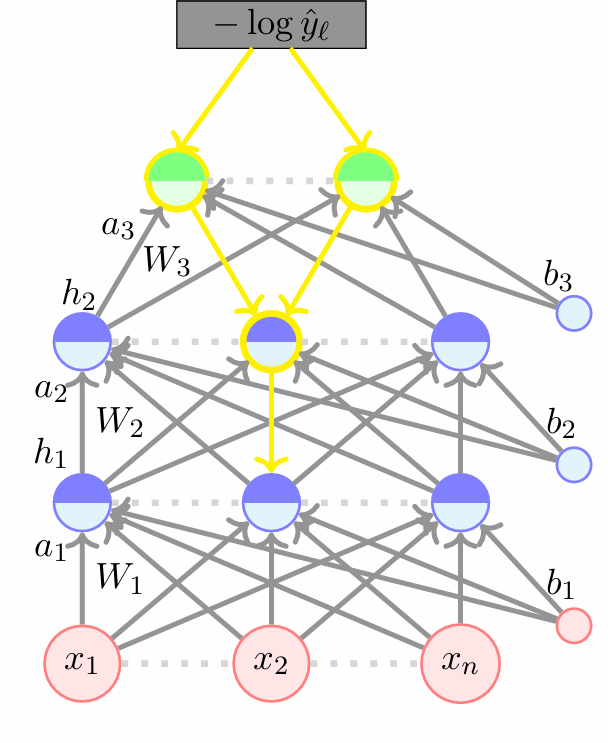
\includegraphics[scale = 0.5]{image_12.png}
\end{minipage}

\begin{align*}
\dfrac{\partial \mathscr{L}(\theta)}{\partial W_{kij}}
&= \dfrac{\partial \mathscr{L}(\theta)}{\partial a_{ki}} \, \dfrac{\partial a_{ki}}{\partial W_{kij}} \\[1.5em]
&= \dfrac{\partial \mathscr{L}(\theta)}{\partial a_{ki}} \, h_{k-1,j}
\end{align*}

\vspace{0.3cm}

\[
\nabla_{W_k} \mathscr{L}(\theta)
=
\begin{bmatrix}
\dfrac{\partial \mathscr{L}(\theta)}{\partial W_{k11}} & \dfrac{\partial \mathscr{L}(\theta)}{\partial W_{k12}} & \cdots & \cdots & \dfrac{\partial \mathscr{L}(\theta)}{\partial W_{k1n}} \\
\vdots & \vdots & \ddots & \ddots & \vdots \\
\vdots & \vdots & \ddots & \ddots & \vdots \\
\vdots & \vdots & \ddots & \ddots & \vdots \\
\dfrac{\partial \mathscr{L}(\theta)}{\partial W_{kn1}} & \dfrac{\partial \mathscr{L}(\theta)}{\partial W_{kn2}} & \cdots & \cdots & \dfrac{\partial \mathscr{L}(\theta)}{\partial W_{knn}}
\end{bmatrix}, \text{ we assume } W_k \in \mathbb{R}^{n \times n}
\]

\vspace{0.3cm}

Lets take a simple example of a $W_k \in \mathbb{R}^{3 \times 3}$ and see what each entry looks like

\[
\nabla_{W_k} \mathscr{L}(\theta) =
\begin{bmatrix}
\dfrac{\partial \mathscr{L}(\theta)}{\partial W_{k11}} & \dfrac{\partial \mathscr{L}(\theta)}{\partial W_{k12}} & \dfrac{\partial \mathscr{L}(\theta)}{\partial W_{k13}} \\[1.5em]
\dfrac{\partial \mathscr{L}(\theta)}{\partial W_{k21}} & \dfrac{\partial \mathscr{L}(\theta)}{\partial W_{k22}} & \dfrac{\partial \mathscr{L}(\theta)}{\partial W_{k23}} \\[1.5em]
\dfrac{\partial \mathscr{L}(\theta)}{\partial W_{k31}} & \dfrac{\partial \mathscr{L}(\theta)}{\partial W_{k32}} & \dfrac{\partial \mathscr{L}(\theta)}{\partial W_{k33}}
\end{bmatrix}
= \dfrac{\partial \mathscr{L}(\theta)}{\partial a_{ki}} \dfrac{\partial a_{ki}}{\partial W_{kij}}
\]

\vspace{0.3cm}

\[
\therefore \nabla_{W_k} \mathscr{L}(\theta) =
\begin{bmatrix}
\textcolor{orange}{\dfrac{\partial \mathscr{L}(\theta)}{\partial a_{k1}}} \, \textcolor{blue}{h_{k-1,1}} &
\textcolor{orange}{\dfrac{\partial \mathscr{L}(\theta)}{\partial a_{k1}}} \, \textcolor{red}{h_{k-1,2}} &
\textcolor{orange}{\dfrac{\partial \mathscr{L}(\theta)}{\partial a_{k1}}} \, \textcolor{red}{h_{k-1,3}} \\[1.5em]

\textcolor{magenta}{\dfrac{\partial \mathscr{L}(\theta)}{\partial a_{k2}}} \, \textcolor{blue}{h_{k-1,1}} &
\textcolor{magenta}{\dfrac{\partial \mathscr{L}(\theta)}{\partial a_{k2}}} \, \textcolor{red}{h_{k-1,2}} &
\textcolor{magenta}{\dfrac{\partial \mathscr{L}(\theta)}{\partial a_{k2}}} \, \textcolor{red}{h_{k-1,3}} \\[1.5em]

\dfrac{\partial \mathscr{L}(\theta)}{\partial a_{k3}} \, \textcolor{blue}{h_{k-1,1}} &
\dfrac{\partial \mathscr{L}(\theta)}{\partial a_{k3}} \, \textcolor{red}{h_{k-1,2}} &
\dfrac{\partial \mathscr{L}(\theta)}{\partial a_{k3}} \, \textcolor{red}{h_{k-1,3}}
\end{bmatrix}
= \nabla_{a_k} \mathscr{L}(\theta) \cdot \utilde{h_{k-1}}^T
\]

\vspace{0.3cm}

\noindent
\begin{minipage}{0.5\textwidth}

Finally, coming to the biases

\[
a_{ki} = b_{ki} + \sum_j W_{kij} h_{k-1,j}
\]

\[
\dfrac{\partial \mathscr{L}(\theta)}{\partial b_{ki}} 
= \dfrac{\partial \mathscr{L}(\theta)}{\partial a_{ki}} \cdot \dfrac{\partial a_{ki}}{\partial b_{ki}}
= \dfrac{\partial \mathscr{L}(\theta)}{\partial a_{ki}}
\]

\vspace{0.2cm}

We can now write the gradient w.r.t. \\ the vector $\utilde{b_k}$.

\[
\nabla_{\mathbf{b}_k} \mathscr{L}(\theta)
=
\begin{bmatrix}
\dfrac{\partial \mathscr{L}(\theta)}{\partial a_{k1}} \\
\dfrac{\partial \mathscr{L}(\theta)}{\partial a_{k2}} \\
\vdots \\
\dfrac{\partial \mathscr{L}(\theta)}{\partial a_{kn}}
\end{bmatrix}
= \nabla_{\mathbf{a}_k} \mathscr{L}(\theta)
\]
\end{minipage}
\hfill
\begin{minipage}{0.5\textwidth}
\centering
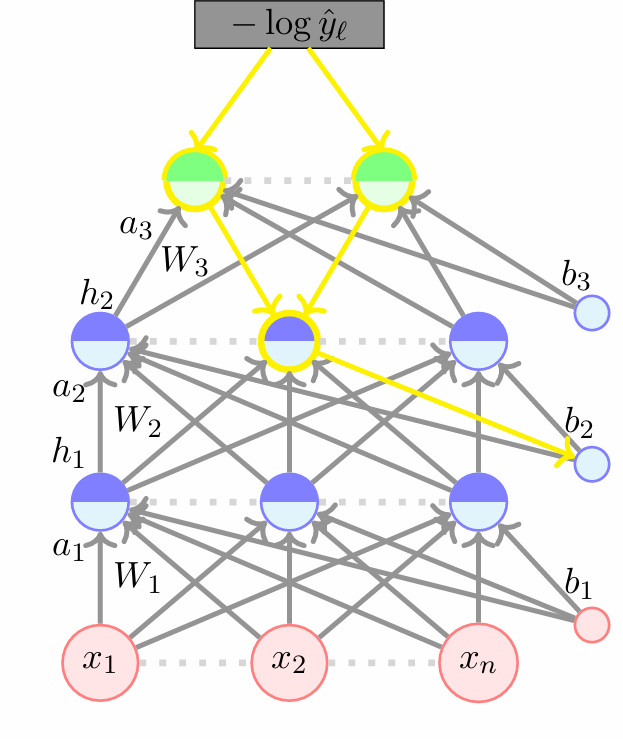
\includegraphics[scale=0.5]{image_13}
\end{minipage}




\section{Summary}

\subsection{for a single data-point}


\begin{itemize}

\item $\nabla W_k = \nabla \utilde{a_k} \cdot \utilde{h_{k-1}}^T$ $\forall$ $k = 1(1)L$

\item $\nabla b_k = \nabla a_k$ $\forall$ $k = 1(1)L$

\item $\nabla a_L = - \left( \utilde{e_{\ell}} - \utilde{\hat{y}} \right)$ 

\item $\nabla a_k = \nabla h_k \odot g'(\utilde{a_k}) = W_{k+1}^T \cdot \nabla a_{k+1} \odot g'(\utilde{a_k})$ $\forall$ $k = 1(1)\overline{L-1}$

\end{itemize}

\newpage

\subsection{for whole $X$}

Given:
\begin{itemize}
    \item \( X \in \mathbb{R}^{n \times m} \) — input data with examples as columns
    \item \( m \) — number of examples
    \item \( L \) — number of layers
\end{itemize}

\noindent The forward propagation equations are:

\begin{itemize}
\item $A_0 = X$

\item $A_k = W_k H_{k-1} + \utilde{b_k} \cdot \mathbf{1}_m^T \quad \forall \; k = 1, 2, \dots, L $


\item $H_k = g_k(A_k) \quad \forall \; k = 1, 2, \dots, L-1$

\item $\hat{Y} = \text{softmax}(A_L)$
\end{itemize}

\noindent The backward propagation equations are:

\begin{itemize}

\item $\nabla W_k = \nabla A_k \cdot H_{k-1}^T $ $\forall$ $k = 1(1) L$

\item $\nabla b_k = \nabla A_k \cdot \mathbf{1}_m$ $\forall$ $k = 1(1) L$ where \( \mathbf{1}_m \in \mathbb{R}^{m \times 1} \) 

\item $\nabla A_L = \frac{1}{m} \left( \hat{Y} - E \right)$ where $E \in \mathbb{R}^{p \times m}$ is the one-hot encoded label matrix for all the data points

\item $\nabla A_k = \nabla H_k \odot g'(A_k) = \left(W_{k+1}^T \cdot \nabla A_{k+1}\right) \odot g'(A_k)$ $\forall$ $k = 1(1)\overline{L-1}$

\end{itemize}




\section{Appendix}

\subsection{Derivative of Activation Function}

\begin{figure}[!htbp]
\centering
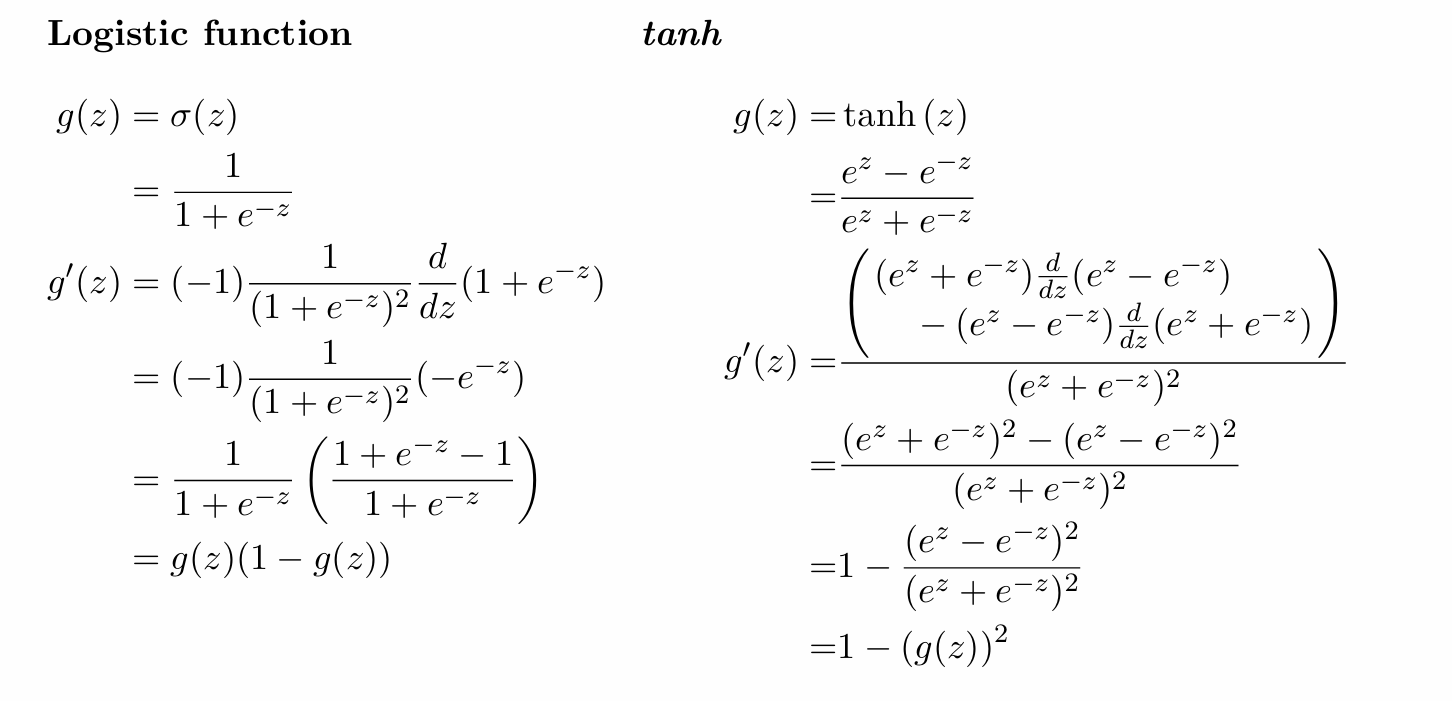
\includegraphics[scale=0.5]{image_14}
\end{figure}

\end{document}